\documentclass[a4paper,11pt]{article}

% Font
\usepackage[T1]{fontenc}
\usepackage[utf8]{inputenc}
\usepackage{lmodern}
\usepackage{tgbonum} % for extra boldness

% Graphics
\usepackage{graphicx}
\usepackage{xcolor}
\usepackage{subcaption}

% Math
\usepackage{amsmath,amssymb,amsthm,textcomp}
\usepackage{enumerate}
\usepackage{multicol}
%\usepackage{tikz}

% Theorem / Proofs
\usepackage{amsthm}
\newtheorem{theorem}{Theorem}

\usepackage{geometry}
\geometry{left=25mm,right=25mm,%
bindingoffset=0mm, top=20mm,bottom=20mm}
\linespread{1.3}

% my own titles
\makeatletter
\renewcommand{\maketitle}{
  \begin{center}
    \vspace{2ex}
    {\huge \textsc{\@title}}
    \vspace{1ex}
    \\
    \@author \hfill \@date
    \vspace{4ex}
  \end{center}
}
\makeatother
%%%

% custom footers and headers
\usepackage{fancyhdr}
\pagestyle{fancy}
\lhead{}
\chead{}
\rhead{}
\lfoot{GeomLab 2020}
\cfoot{}
\rfoot{Page \thepage}
\renewcommand{\headrulewidth}{0pt}
\renewcommand{\footrulewidth}{0pt}
%

% code listing settings
\usepackage{listings}
\lstset{
  language=Python,
  basicstyle=\ttfamily\small,
  aboveskip={1.0\baselineskip},
  belowskip={1.0\baselineskip},
  columns=fixed,
  extendedchars=true,
  breaklines=true,
  tabsize=4,
  prebreak=\raisebox{0ex}[0ex][0ex]{\ensuremath{\hookleftarrow}},
  frame=lines,
  showtabs=false,
  showspaces=false,
  showstringspaces=false,
  keywordstyle=\color[rgb]{0.627,0.126,0.941},
  commentstyle=\color[rgb]{0.133,0.545,0.133},
  stringstyle=\color[rgb]{01,0,0},
  numbers=left,
  numberstyle=\small,
  stepnumber=1,
  numbersep=10pt,
  captionpos=t,
  escapeinside={\%*}{*)}
}

% No paragraph indentation
\setlength{\parindent}{0in}

% ----------------------
\begin{document}
% ----------------------

\title{GeomLab 2020}
\author{}
\date{\today}
\maketitle

% ----------------------
\tableofcontents
% ----------------------

\newpage

% ----------------------
\section{Motivation}
% ----------------------

Motivated by the COVID-19 disease several outlets printed two-dimensional depictions of data which usually contained multidimensional datasets. These datasets usually compromise \{\textit{infections, recoverd, death}\} rates with regard to the \textit{country} and sometimes also the evolution over \textit{time}.\\

\begin{figure}[h]
  \begin{subfigure}{0.5\textwidth}
    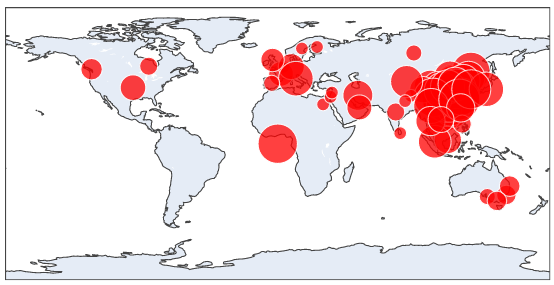
\includegraphics[width=0.9\linewidth]{covid_spread_20200223.png}
    \caption{23.02.2020}\label{fig:covid2020Feb}
  \end{subfigure}
  \begin{subfigure}{0.5\textwidth}
    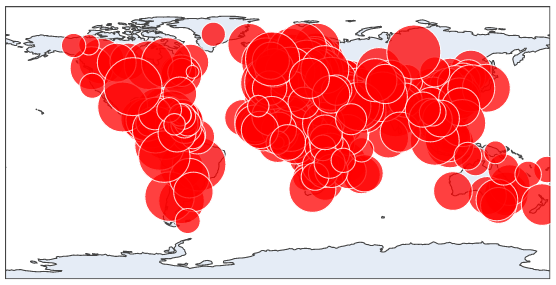
\includegraphics[width=0.9\linewidth]{covid_spread_20200511.png}
    \caption{11.05.2020}\label{fig:covid2020May}
  \end{subfigure}
  \caption{Comparison of a typical scatterplot depicting the $log$ of confirmed cases as the radius.}
  \label{fig:covid19}
\end{figure}

In this lab we focus on depicting data in a meaningful way. Besides its quantitative nature this task has some qualitative properties. Similar to many solutions of problems in computational geometry, like deciding if a point is contained in a polygon or the construction of a convex hull for a set of points, the quality of the scatterplot is obvious to the human observer. Not so for a machine. While Fig. (\ref{fig:covid2020Feb}) is highly informative for a human or potential policy maker, Fig. (\ref{fig:covid2020May}) bears little information content. Despite this fact both figures result from the very same algorithm depicting data from the disease spread of COVID-19 during 2020 [Algo im Appendix].\\

To investigate the quantification of visual quality mainly Tufte in 1983 in \textit{The visual display of quantitative information graphics press"} and Miller et al in \textit{The Need For Metrics In Visual Information Analysis} provided fundamental work. Based on this, follow-up work and further considerations from visibility problems and sorting we develop a novel approach to visualize multidimensional data in a scatterplot which transports as much information content as possible.

\newpage

% ----------------------
\section{Problem Statement and State of the Art}
% ----------------------

\subsection{Problem statement and constraints}

\begin{enumerate}
  \item Represention and visibility of scatter plots with glyphs
  \item Represention and visibility of multi-dimensional data in nested discs
  \item Represention and visibility of pie charts glyphs
  \item Represention and visibility of (one?) other type of glyphs
\end{enumerate}

\subsection{Previous work}

\begin{enumerate}
  \item See papers in Slack Channel
\end{enumerate}

\newpage
\section{Methodology}

\subsection{Cost functions}

\begin{enumerate}
  \item Information content covered by the data,
  \item information content of the data in the visualization,
  \item information capacity of a visualization,
  \item topological information content.
\end{enumerate}



\subsection{Selection of algorithms and complexity}

\begin{enumerate}
  \item Random inseration
  \item Painter
  \item MaxMinSumK/absolute - Sum of visible circumference/hull
  \item MaxMinSumK/weighted - weighted such that big circles/glyphs not dominate
  \item MaxMinSumK/relative - Sum of relative circumference/hull
  \item MaxMinMinK/absolute - MaxMin of minimal visible circumference/hull of each circle/glyph
  \item MaxMinMinK/relative
\end{enumerate}

\subsection{Optimalitaet fuer Pie Chart}

Let $D$ be a finite set and for $d \in D$ and $S \subseteq D$ the function $ \phi(d, S) \mapsto \Re_{\geq 0} $ with the property, that for every $d \in D$ $S' \subseteq S => \phi(d, S') \geq \phi(d, S)$.

Let the stacking-order $\pi: \{1,...,n\} \mapsto D$ be bijective.

\begin{theorem}
  
The algorithm

\begin{verbatim}
ALG(finite set D) {
  x := argmax_{d \in D} \phi(d, D \setminus {d})
  return [x, ALG(D \setminus {x})]
}
\end{verbatim}

returns a stacking-order, which maximizes $min_{d \in D} \phi(d, \{d\ \in D | d' > d\})$. \textbf{Roland: shouldn't it be minimizes?}
\end{theorem}

\begin{proof}
  Given an optimal Stacking-Order $s$ and output of ALG $s^*$ .

  \begin{enumerate}
    \item case: $s=s^*$. Done.
    \item case: $s \neq s^*$. $s \neq s^*$ implies, that there is a lowest $k \in N$, such that $s(k) \neq s^*(k)$. Let $s(k) = d_k$ and $s^* = d^*_k$. Hence, $k^* = s^{-1}(s^*(k)) = s^{-1}(d^*_k)$ is the index of $d^*_k$ with respect to $s$. It follows $k<k^*$.
  \end{enumerate}
\end{proof}

\begin{enumerate}
  \item Rotation
  \item Physics/Heuristics based approaches
\end{enumerate}

\begin{figure}[htp]
  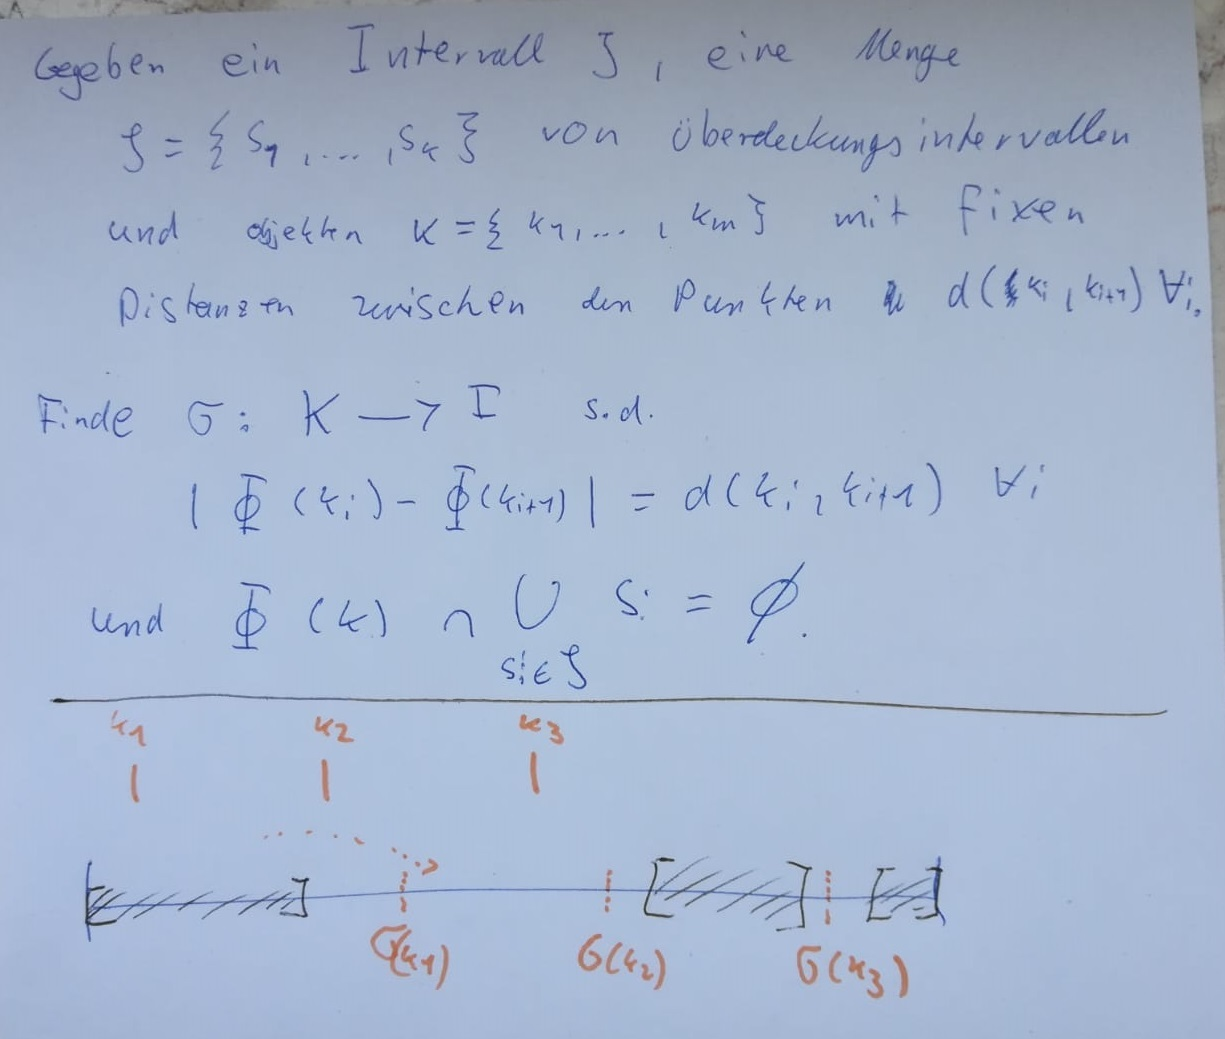
\includegraphics[width=\textwidth,height=\textheight,keepaspectratio]{assets/trennlinienproblem.jpg}
  \caption{Trennlinienproblem}
\end{figure}

\newpage

% ----------------------
\section{Experimental validation}
% ----------------------

\begin{figure}[htp]
  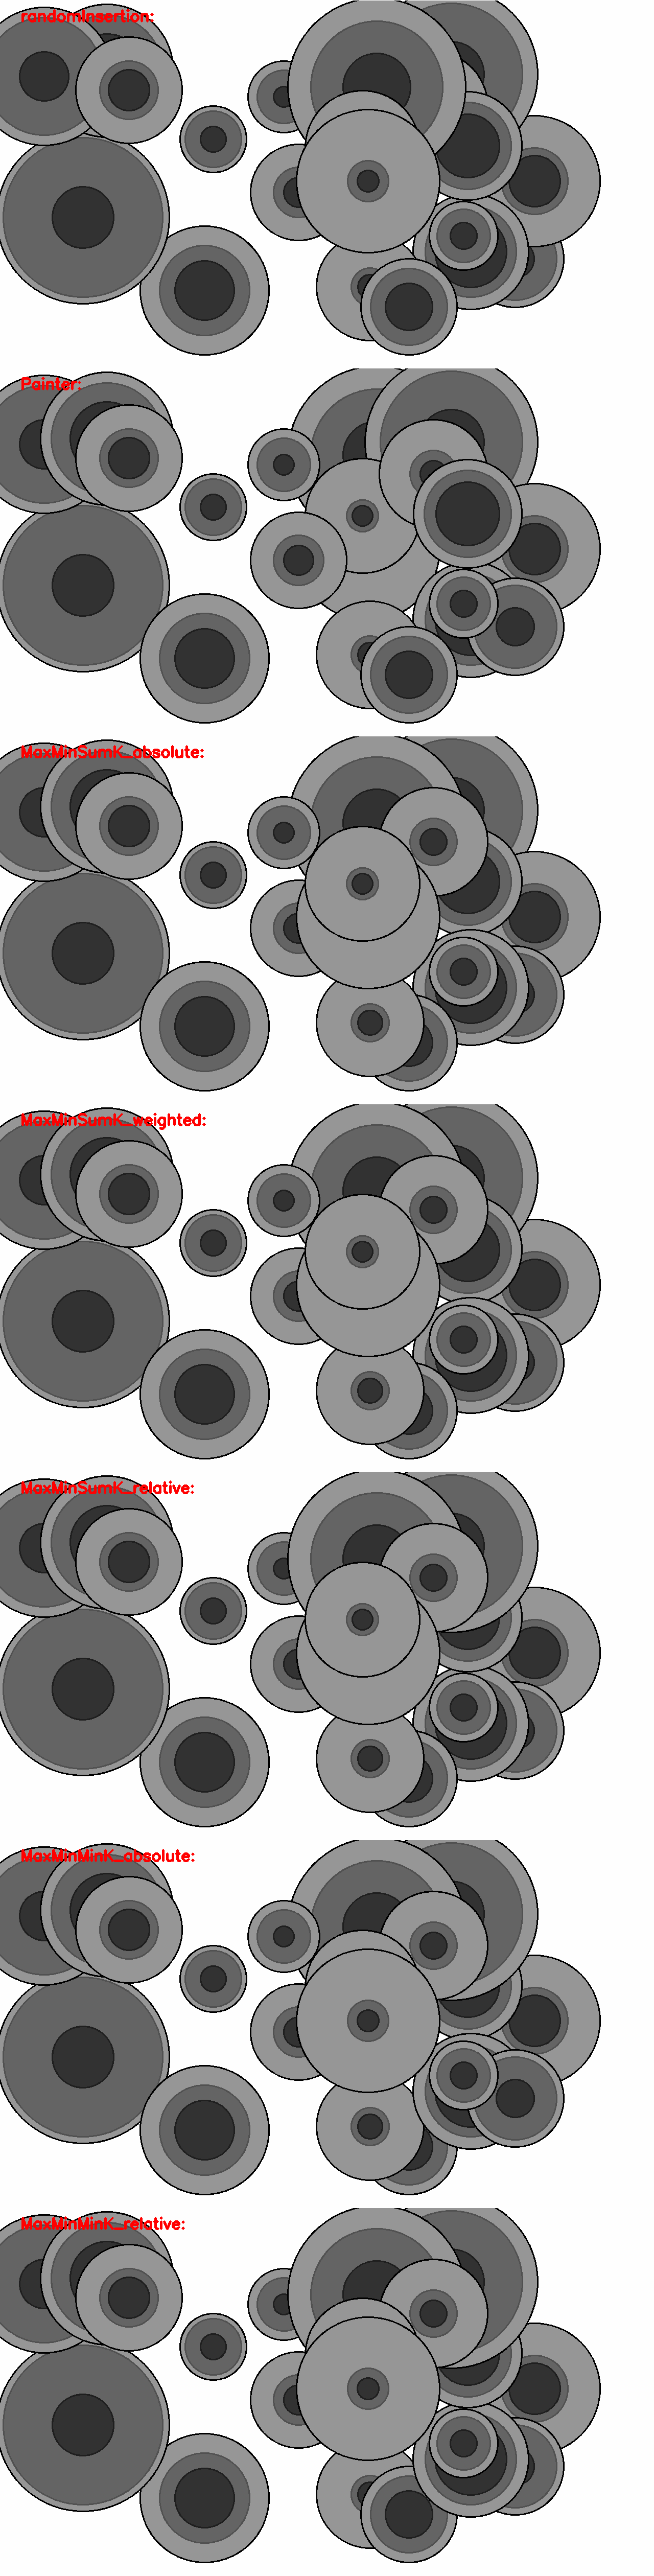
\includegraphics[width=\textwidth,height=0.7\textheight,keepaspectratio]{assets/cost_functions.png}
\end{figure}

\begin{figure}[htp]
  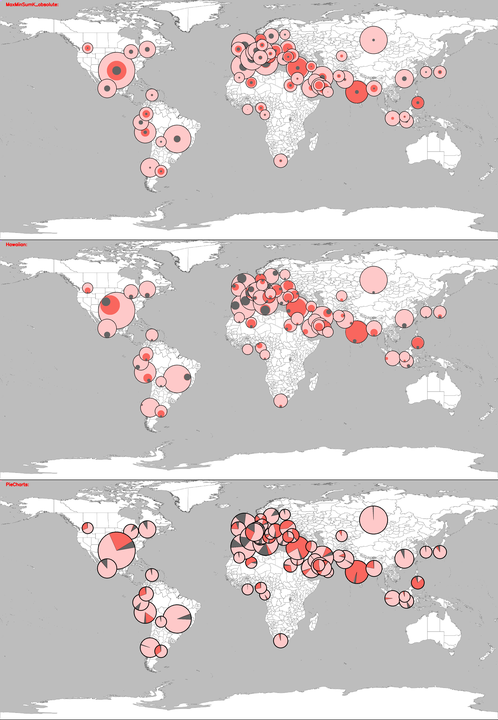
\includegraphics[width=\textwidth,height=\textheight,keepaspectratio]{assets/covid19_nested_discs.png}
\end{figure}

\begin{figure}[htp]
  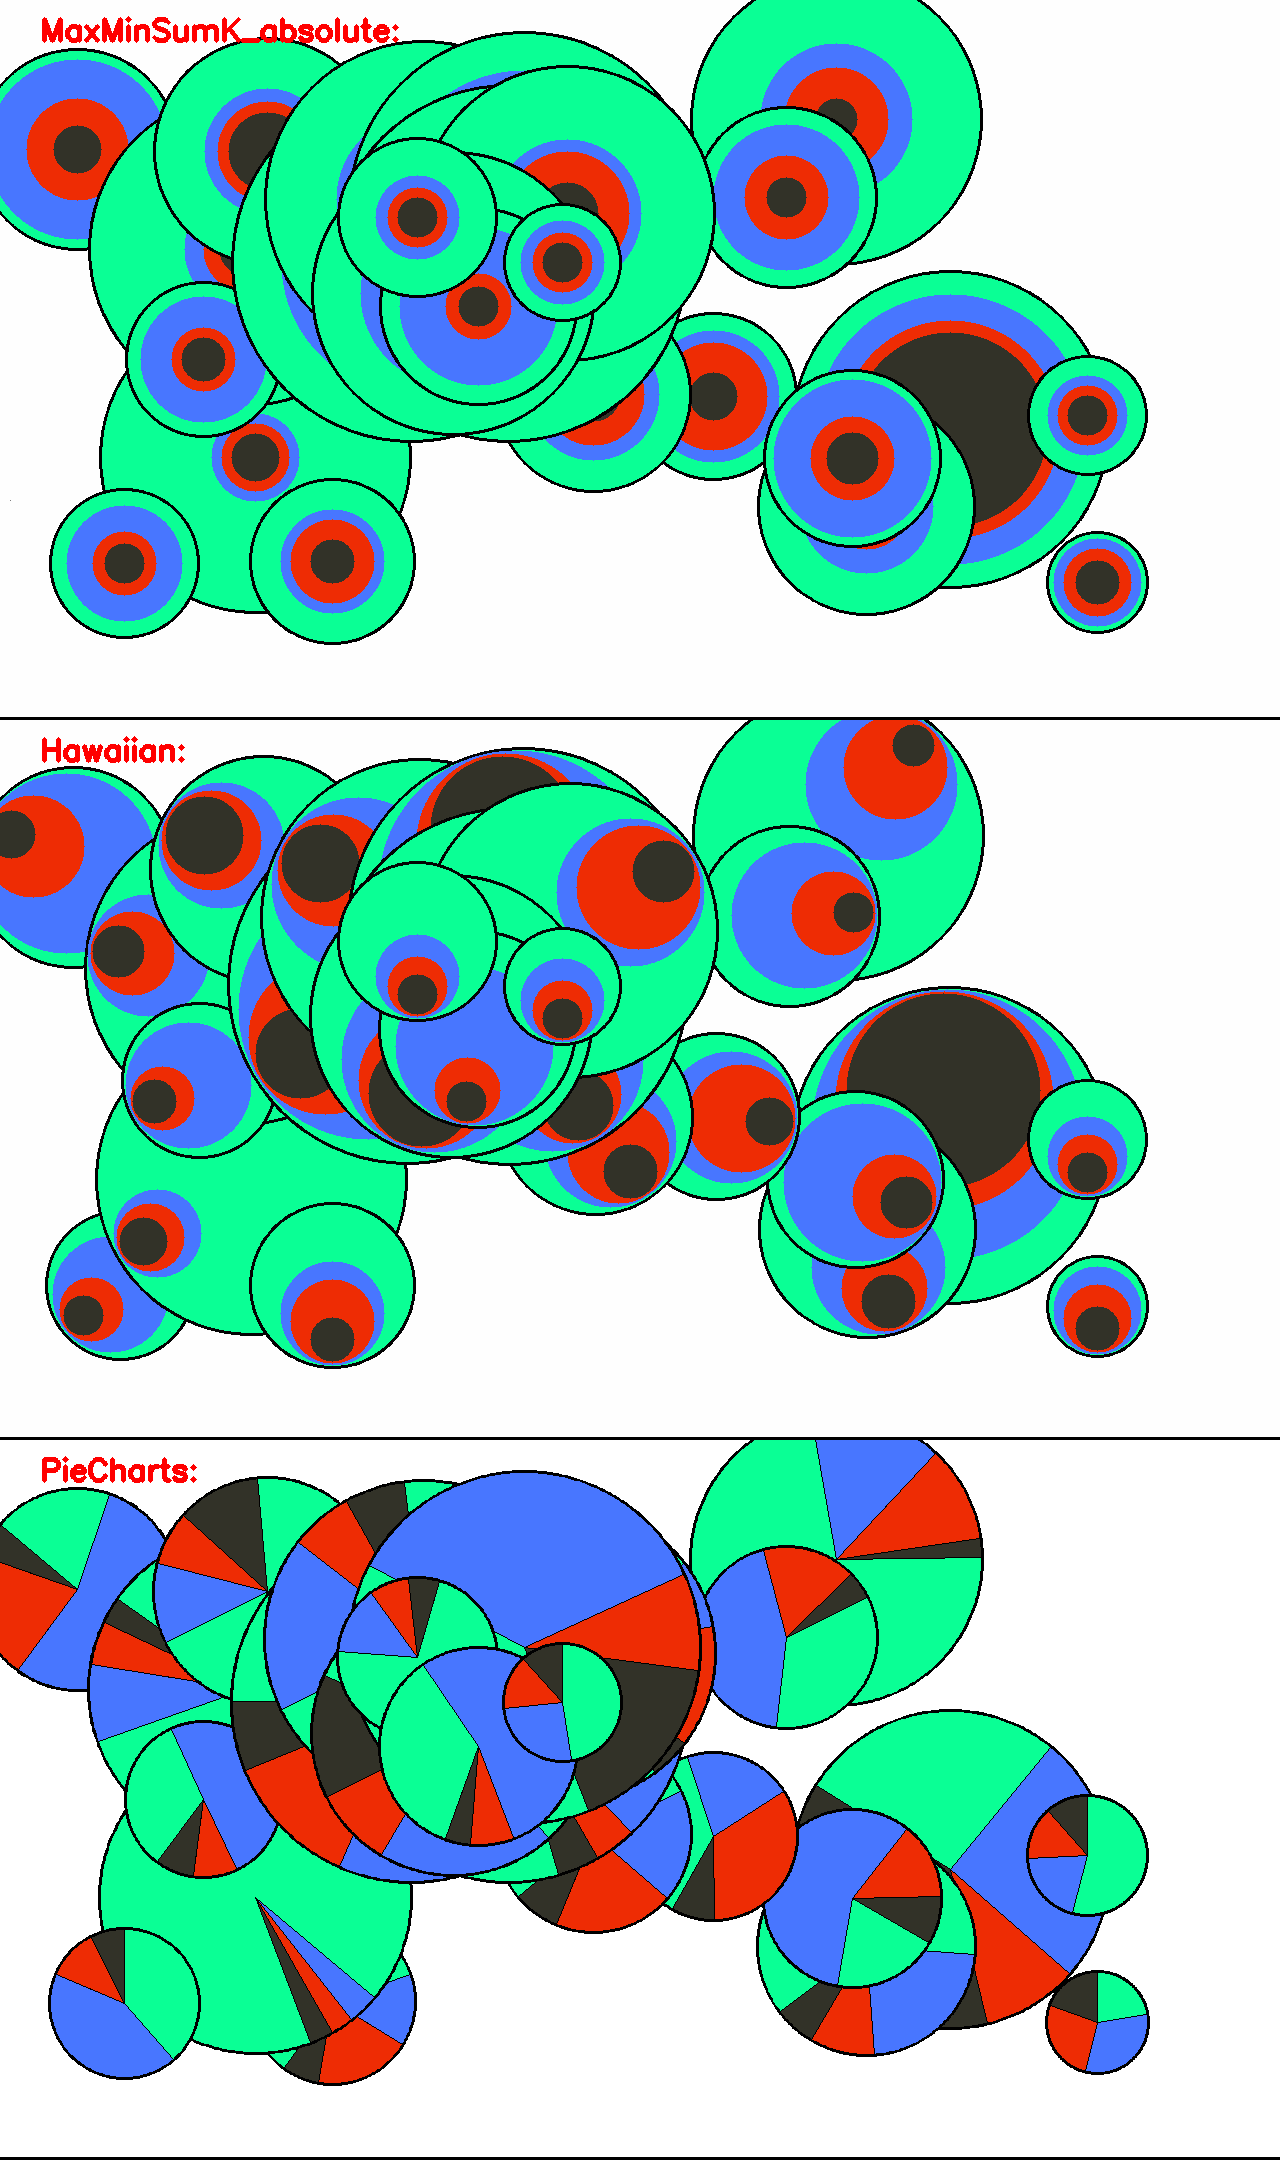
\includegraphics[width=\textwidth,height=\textheight,keepaspectratio]{assets/nested_discs_all.png}
\end{figure}

\newpage


\section{Sources}


Tufte, Edward R. "The visual display of quantitative information graphics press." Cheshire, Connecticut (1983).\\

Miller, Nancy, et al. "The need for metrics in visual information analysis." Proceedings of the 1997 workshop on New paradigms in information visualization and manipulation. 1997.\\

Brath, Richard. "Metrics for effective information visualization." Proceedings of VIZ'97: Visualization Conference, Information Visualization Symposium and Parallel Rendering Symposium. IEEE, 1997.\\

Tatu, Andrada, et al. "Visual quality metrics and human perception: an initial study on 2D projections of large multidimensional data." Proceedings of the International Conference on Advanced Visual Interfaces. 2010.\\

Urribarri, D. K., \& Castro, S. M. (2016). Prediction of data visibility in two-dimensional scatterplots. Information Visualization, 16(2), 113–125. doi:10.1177/1473871616638892\\

Coeurjolly, D., Miguet, S., \& Tougne, L. (2004). 2D and 3D visibility in discrete geometry: an application to discrete geodesic paths. Pattern Recognition Letters, 25(5), 561–570. doi:10.1016/j.patrec.2003.12.002\\

Yang-Pelaez J and Flowers WC. Information content
measures of visual displays. In: Proceedings of the IEEE symposium on information vizualization 2000 (INFOVIS’00), 2000, pp. 99–103. Washington, DC: IEEE Computer Society.


\end{document}

% code from http://rosettacode.org/wiki/Fibonacci_sequence#Python
\begin{lstlisting}[label={list:first},caption=Sample Python code -- Fibonacci sequence calculated analytically.]
from math import *

# define function 
def analytic_fibonacci(n):
  sqrt_5 = sqrt(5);
  p = (1 + sqrt_5) / 2;
  q = 1/p;
  return int( (p**n + q**n) / sqrt_5 + 0.5 )

# define range
for i in range(1,31):
  print analytic_fibonacci(i)
\end{lstlisting}

Following Listing~\ref{list:first}\ldots{} 

Tufte proposed to measure quality based on the amount of consumed ink and purpose of the ink. He stated that the majority of the used ink in a graph must represent information about the data. Most recently Tatu et al. showed "that quality measures can simulate the selection of best views by human beings." and also compares a set of promising and established measures. In the motivated usecase, especially scatterplots using glyphs like circles or discs are of major interest, because of their advantages when plotting multidimensional data [Tatu et al.].\\

In a first step, following the common depiction, we consider circles as glyph. Further, we assume that the data $\mathcal{D}$ is finite and three-dimensional. We map two dimensions to the location $(x_i, y_i)$ and the remaining one dimension of our data set to the radius $r_i$ of a circle $C_i$, i.e., $ (x_i, y_i, r_i) \in \mathcal{D} \subset \mathbb{R}^3$. Moreover, we ignore transparency and other means to circumvent the occlusion of circles overlaying each other.\\

As already mentioned in the Motivation we want to maximize visibility of the data. Urribari et al define visibility as
%
\begin{equation} \label{eq1}
  \begin{split}
    visiblity & = 1 - occlusion \\
              & = f(data(set), visualization \, parameters)\\
  \end{split}
\end{equation}
%
with $occlusion$ being defined as [Tatu et al.]:
%
\begin{equation}
  occlusion = { \text{no. of data points completely occluded } \over \text{total no. of data points}}\\
\end{equation}

Using this simple definition it is possible to formulate two equivalent cost functions already now:
%
\begin{equation} \label{eq3}
  \begin{split}
    \min\limits_{\text{vis. par.}} & \; occlusion\\
    \max\limits_{\text{vis. par.}} & \; visiblity\\
  \end{split}
\end{equation}
%
We focus on visiblity for now. When using circles as glyphs, we can split the visibilty in two components:
%
\begin{equation} \label{eq3}
  \begin{split}
    U_i = & \delta C_i \, \setminus \bigcup_{D} C_j\\
    A_i = & \, C_i \; \setminus \bigcup_{D} C_j\\
  \end{split}
\end{equation}
%
and sum over the visible circumferences and areas
%
\begin{equation} \label{eq3}
  \begin{split}
    U_{occlusion} & = \sum_i U_i\\
    A_{occlusion} & = \sum_i A_i\\
  \end{split}
\end{equation}
%
which already hints toward potential cost functions.\\

Here many variations and specific options are thinkable. Like considering (1) relative circumference to circle area, (2) relative area to circumference, etc.
